%
\documentclass[12pt]{article}

\usepackage{fullpage}
\usepackage{setspace}
\usepackage{endnotes}
\usepackage{amsmath}
\usepackage{amsfonts}
\usepackage{amssymb}
\usepackage{mathrsfs}
\usepackage{calrsfs}
\usepackage{rotating}
\usepackage{dcolumn}
\usepackage{longtable}
\usepackage{microtype}
\usepackage{graphicx}
\usepackage{url}
\usepackage{natbib}
\bibpunct{(}{)}{;}{a}{}{,}
\usepackage{framed}
\usepackage{lipsum}
\usepackage[font=small,labelfont=sc]{caption}
 \usepackage{float}
\restylefloat{table}
\usepackage[usenames,dvipsnames]{color}

% refs and pdf meta
\usepackage{hyperref}
\hypersetup{
 pdftitle={Dealing with Separation in Logistic Regression Models}, % title
 pdfauthor={Carlisle Rainey}, % author
 pdfkeywords={logistic regression}{separation}{Firth}{Cauchy}{MCMC}
 pdfnewwindow=true, % links in new window
 colorlinks=true, % false: boxed links; true: colored links
 linkcolor=black,%BrickRed, % color of internal links
 citecolor=black, % color of links to bibliography
 filecolor=black, % color of file links
 urlcolor=blue % color of external links
}

% Set up theorems, etc.
\usepackage{amsthm}
\newtheorem{lemma}{Lemma}
\newtheorem{proposition}{Proposition}
\newtheorem{theorem}{Theorem}
\newtheorem{claim}{Claim}
\newtheorem{assumption}{Assumption}
\newtheorem{defn}{Definition}

% Allow restating theorems (for the Appendix)
\usepackage{thmtools}
\usepackage{thm-restate}
\usepackage{cleveref}

% Set up fonts the way I like
\usepackage{tgpagella}
\usepackage[T1]{fontenc}
%\usepackage[T1]{fontenc}
\usepackage[bitstream-charter]{mathdesign}

%Redefine the first level
\renewcommand{\theenumi}{\arabic{enumi}.}
\renewcommand{\labelenumi}{\theenumi}
%Redefine the second level
\renewcommand{\theenumii}{\alph{enumii}.}
\renewcommand{\labelenumii}{\theenumii}
%Redefine the third level
\renewcommand{\theenumiii}{\roman{enumiii}.}
\renewcommand{\labelenumiii}{\theenumiii}
%Redefine the fourth level
\renewcommand{\theenumiv}{\Alph{enumiv}.}
\renewcommand{\labelenumiv}{\theenumiv}

\parskip=0pt
\parindent=20pt
\usepackage{lscape}
\singlespace

% Create footnote command so that my name
% has an asterisk rather than a one.
\long\def\symbolfootnote[#1]#2{\begingroup%
\def\thefootnote{\fnsymbol{footnote}}\footnote[#1]{#2}\endgroup}

\begin{document}

\begin{center}
{\Large Dealing with Separation in Logistic Regression Models\symbolfootnote[1]{I thank Mark Bell and Nicholas Miller for making their data available \citep{bell-miller-data}.
I thank Mike Alvarez, Mark Bell, Bryce Corrigan, David Firth, Paul Johnson, Nicholas Miller, Jamie Monogan, Chris Zorn, and two anonymous reviewers for helpful comments. 
I presented earlier versions of this paper at the University of Kansas, Texas A\&M University, the 2015 annual meeting of The Society for Political Methodology, and the 2016 Annual Meeting of the Southern Political Science Association. The analyses presented here were conducted with \texttt{R} 3.2.2. All data and computer code \citep{separation-data} necessary for replication are available at \href{https://github.com/carlislerainey/priors-for-separation}{github.com/carlislerainey/priors-for-separation} and on the Political Analysis Dataverse at \href{http://dx.doi.org/10.7910/DVN/VW7G2Q}{dx.doi.org/10.7910/DVN/VW7G2Q}. %The R package \texttt{separation} (currently version 0.1, alpha pre-release) implements the procedures discussed in the paper and is available at \href{https://github.com/carlislerainey/separation}{github.com/carlislerainey/separation}. See the \href{https://github.com/carlislerainey/separation/blob/master/README.md}{README} for instructions on downloading and usage.
}
}

\vspace{10mm}

Carlisle Rainey\symbolfootnote[2]{Carlisle Rainey is Assistant Professor of Political Science, Texas A\&M University, 2010 Allen Building, College Station, TX, 77843 (\href{mailto:crainey@tamu.edu}{crainey@tamu.edu}).}

\end{center}

% remove page number from first page
\thispagestyle{empty}

%\begin{center}
%\begin{footnotesize}
%\today\\
%\vspace{3mm}
%Working paper: Comments welcome!
%\end{footnotesize}
%\end{center}

% abstract
\vspace{10mm}
{\centerline{\textsc{Abstract}}}
\begin{quote}
\noindent When facing small numbers of observations or rare events, political scientists often encounter separation, in which explanatory variables perfectly predict binary events or non-events. 
In this situation, maximum likelihood provides implausible estimates and the researcher might want incorporate some form of prior information into the model. 
The most sophisticated research uses Jeffreys' invariant prior to stabilize the estimates. 
While Jeffreys' prior has the advantage of being automatic, I show that it often provides too much prior information, producing smaller point estimates and narrower confidence intervals than even highly skeptical priors. 
To help researchers assess the amount of information injected by the prior distribution, I introduce the concept of a partial prior distribution and develop the tools required to compute the partial prior distribution of quantities of interest, estimate the subsequent model, and summarize the results.
\end{quote}

%\vspace{10mm}
%\begin{center}
%Word Count: 7,751
%\end{center}

\newpage
\doublespace

Separation, in which an explanatory variable perfectly predicts some binary observations, remains a hurdle in political science research (e.g., \citealt{BellMiller2015}; \citealt{Mares2015}; \citealt{ViningWilhelmCollens2015}; \citealt{BrownKaplow2014}; \citealt{BarrilleauxRainey2014};  \citealt{LeemanMares2014}; \citealt{Reiter2014}; \citealt{Weisiger2014}; \citealt{MinozziVolden2013}; \citealt{CedermeanGleditschHug2013}; \citealt{Fuhrmann2012}; \citealt{RoccaSanchezMorin2011}; \citealt{PetersonDrury2011}; \citealt{CoxKousserMcCubbins2010}; \citealt{Ahlquist2010}; \citealt{Rauchhaus2009}; \citealt{SmithFridkin2008}; \citealt{Casellas2008}; \citealt{DesposatoScheiner2008}; \citealt{HellerMershon2008}; \citealt{DeRouenBercovitch2008}).
\cite{Zorn2005} offers the most principled solution to the problem of separation, suggesting that researchers maximize a penalized version \citep{Firth1993} of the usual likelihood function (see also \citealt{HeinzeSchemper2002}). 
Zorn's approach has the advantage of being automatic and easy for researchers to use.

However, when implementing Zorn's approach, substantive researchers face two major problems. 
First, because the posterior distribution of the coefficients can be highly non-normal under separation, the usual asymptotic confidence intervals and $p$-values do not work well. 
While a good method exists for finding confidence intervals and $p$-values for the model coefficients \citep{HeinzeSchemper2002}, this method does not extend to the typical quantities of interest, such as first differences. 
Researchers must still rely on the poor asymptotic approximation to simulate these quantities \citep{KingTomzWittenberg2000}.  
Secondly, and perhaps most importantly, while the penalty suggested by Zorn has the attractive property of bias reduction in logistic regression models \citep{Firth1993}, it does not necessarily approximate a researcher's prior information (\citealt{WesternJackman1994} and \citealt{Gelmanetal2008}). 
Some shrinkage toward zero is required to obtain finite estimates, but the appropriate amount of shrinkage depends on the substantive problem and the prior information. 
To address these two problems, I suggest that researchers use a range of priors, focusing on an informative prior, and use MCMC to simulate directly from the posterior.

In this paper, I introduce conceptual and computational tools that help researchers understand the information provided by a given prior distribution and use that prior distribution to obtain meaningful point estimates and confidence intervals. 
I make three specific contributions. 
First, I use statistical theory and two applied examples to demonstrate the importance of choosing a prior distribution that represents actual prior information and conducting robustness checks using a variety of prior distributions. 
Second, I introduce the concept of a partial prior distribution, a powerful tool in understanding and choosing a prior when facing separation. 
Third, I introduce new software that makes it easy for researchers to choose an informative prior distribution, simulate directly from the posterior distribution, and summarize the inferences.%\footnote{
%The R package \texttt{separation} (currently version 0.1, alpha pre-release) implements the procedures discussed in the paper and is available at \href{https://github.com/carlislerainey/separation}{github.com/carlislerainey/separation}. 
%See the \href{https://github.com/carlislerainey/separation/blob/master/README.md}{README} for instructions on downloading and usage.}

I begin with a basic overview of the logistic regression model and summary of the impact of separation on the maximum likelihood estimates. 
I then describe two default prior distributions that researchers might use to handle separation. 
Next, I use a theoretical result and an applied example to demonstrate the importance of choosing an informative prior. 
I then introduce researchers to the concept of a partial prior distribution, which enables researchers to understand complex prior distributions in terms of the key quantities of interest. 
To illustrate how these ideas work in practice, I conclude with a replication of \cite{Rauchhaus2009} and \cite{BellMiller2015}, whose disagreement about the effect of nuclear weapons on war hinges, in part, on how to deal with separation.

\section*{The Logistic Regression Model}

Political scientists commonly use logistic regression to model the probability of events such as war (e.g., \citealt{Fearon1994}), policy adoption (e.g., \citealt{BerryBerry1990}), turning out to vote (e.g., \citealt{WolfingerRosenstone1980}), and government formation (e.g., \citealt{MartinStevenson2001}). 
In the typical situation, the researcher uses an $n \times (k + 1)$ design matrix $X$ consisting of a single column of ones and $k$ explanatory variables to model a vector of $n$ binary outcomes $y$, where $y_i \in \{0, 1\}$, using the model $\text{Pr}(y_i) = \text{Pr}(y_i = 1~|~ X_i) = \dfrac{1}{1 + e^{-X_i\beta}}$, where $\beta$ is a coefficient vector of length $k + 1$. 

Using this model, it is straightforward to calculate the likelihood function 
\begin{equation}
\text{Pr}(y | \beta) = L(\beta | y) = \displaystyle \prod_{i = 1}^n \left[\left( \dfrac{1}{1 + e^{-X_i\beta}}\right)^{y_i}\left(1 - \dfrac{1}{1 + e^{-X_i\beta}}\right)^{1 - y_i}\right]\text{.}
\end{equation}
Researchers routinely obtain the maximum likelihood estimate $\hat{\beta}^{mle}$ of the coefficient vector $\beta$ by finding the coefficient vector that maximizes $L$ (i.e., maximizing the likelihood of the observed data). 
While this approach works quite well in most applications, it fails in a situation known as separation \citep{Zorn2005}.

\section*{Separation}

Separation occurs in models of binary outcome data when one explanatory variable perfectly predicts zeros, ones, or both.\footnote{
Separation can also occur when a \emph{combination} of explanatory variables perfectly predicts zeros, ones, or both, see \cite{LesaffreAlbert1989}. 
See \cite{Geyer2009} for a much more general view of the concept of separation.} 
For a binary explanatory variable $s_i$ (for \underline{s}eparating explanatory variable), \textit{complete separation} occurs when $s_i$ perfectly predicts \emph{both} zeros \emph{and} ones.\footnote{
For simplicity, I describe complete and quasicomplete separation for a \textit{binary} explanatory variable, which is more explicable than the general case considered by \cite{AlbertAnderson1984}. 
My approach also follows the convention of \cite{HeinzeSchemper2002} and \cite{Zorn2005}. 
Indeed, in social science problems, binary explanatory variables more commonly lead to separation, so little is lost.} 
\textit{Quasicomplete separation} occurs when $s_i$ perfectly predicts \emph{either} zeros \emph{or} ones, but not both (\citealt{AlbertAnderson1984} and \citealt{Zorn2005}). 
\textit{Overlap}, the ideal case, occurs when there is no such $s_i$. 
With overlap, the usual maximum likelihood estimates exist and provide reasonable estimates of parameters. 
However, under complete or quasicomplete separation, finite maximum likelihood estimates do not exist and the usual method of calculating standard errors fails (\citealt{AlbertAnderson1984} and \citealt{Zorn2005}).

For the binary explanatory variable $s_i$, complete separation occurs when $s_i$ perfectly predicts \emph{both} zeros \emph{and} ones. 
For example, suppose $s_i$, such that $y_i = 0$ for $s_i = 0$ and $y_i = 1$ for $s_i = 1$. 
To maximize the likelihood of the observed data, the ``S''-shaped logistic regression curve must assign $\text{Pr}(y_i) = \frac{1}{1 + e^{-X_i\beta}} = 0$ when $s_i  = 0$ and $\text{Pr}(y_i) = \frac{1}{1 + e^{-X_i\beta}} = 1$ when $s_i = 1$. 
Since the logistic regression curve lies strictly between zero and one, this likelihood cannot be achieved, only approached asymptotically as the coefficient $\beta_s$ for $s_i$ approaches infinity. 
Thus, the likelihood function under complete separation is monotonic, which implies that a finite maximum likelihood estimate does not exist.

Quasicomplete separation occurs when $s_i$ perfectly predicts \emph{either} zeros \emph{or} ones.
For example, suppose that when $s_i = 0$, sometimes $y_i = 1$ and other times $y_i = 0$, but when $s_i = 1$, $y_i = 1$ \emph{always}. 
To maximize the likelihood of the observed data, the ``S''-shaped logistic regression curve must assign $\text{Pr}(y_i) = \frac{1}{1 + e^{-X_i\beta}} \in (0, 1)$ when $s_i  = 0$ and $\text{Pr}(y_i) = \frac{1}{1 + e^{-X_i\beta}} = 1$ when $s_i = 1$. 
Again, since the logistic regression curve lies strictly between zero and one, this likelihood cannot be achieved, only approached asymptotically. 
Thus, the likelihood function under quasicomplete separation also monotonically increases as the coefficient of $s_i$ increases, which again implies that the maximum likelihood estimate does not exist.

For example, \cite{BarrilleauxRainey2014} find that no Democratic governors opposed the Medicaid expansion under the Affordable Care Act, leading to a maximum likelihood estimate of negative infinity for the coefficient of the indicator of Democratic governors. 
Similarly, \cite{Rauchhaus2009} (see \citealt{BellMiller2015}) finds no instances of states with nuclear weapons engaging in war with each other, leading to an estimated coefficient of negative infinity for the coefficient of the variable indicating nuclear dyads. 
To maximize the likelihood in these situations, the model must assign zero probability of opposition to Democratic governors and zero probability of war to nuclear dyads. 
Because the logistic regression curve lies strictly above zero, this cannot happen, though it can be approached asymptotically as the coefficient of $s_i$ goes to negative infinity. 

For convenience, I say that the ``direction of the separation'' is positive if and only if $s_i = 1 \implies y_i = 1$ \underline{or} $s_i = 0 \implies y_i = 0$ and that the direction of separation is negative if and only if $s_i = 0 \implies y_i = 1$ \underline{or} $s_i = 1 \implies y_i = 0$. 
Thus, $\hat{\beta}^{mle} = +\infty$ when the direction of the separation is positive, and $\hat{\beta}^{mle} = -\infty$ when the direction of the separation is negative.

\section*{Solutions to Separation}

The maximum likelihood framework requires the researcher to find the parameter vector that ``maximizes the likelihood of the observed data.'' 
Of course, infinite coefficients \textit{always} generate separated data, while finite coefficients only \emph{sometimes} generate separation. 
Thus, under separation, maximum likelihood can only produce infinite estimates.

Before addressing potential solutions to this problem, let me mention two unsatisfactory ``solutions'' found in applied work. 
In some cases, researchers simply ignore the problem of separation and interpret the large estimates and standard errors as though these are reasonable. 
However, this approach leads researchers to overstate the magnitude of the effect and the uncertainty of the estimates. 
Secondly, researchers sometimes ``solve'' the problem of separation by dropping the separating variable from the model. 
\citet[pp. 161-162]{Zorn2005} correctly dismisses this approach:
\begin{quote}
As a practical matter, separation forces the analyst to choose from a number of problematic alternatives for dealing with the problem. The most widely used ``solution'' is simply to omit the offending variable or variables from the analysis. In political science, this is the approach taken in a number of studies in international relations, comparative politics, and American politics. It is also the dominant approach in sociology, economics, and the other social sciences, and it is the recommended method in a few prominent texts in statistics and econometrics. Of course, this alternative is a particularly unattractive one; omitting a covariate that clearly bears a strong relationship to the phenomenon of interest is nothing more than deliberate specification bias.
\end{quote}

One principled solution is to build prior information $p(\beta)$--the same prior information that leads researchers to deem infinite coefficients ``implausibly large''--into the model using Bayes' rule, so that 
\begin{equation}
p(\beta|y) = \dfrac{\overbrace{p(y|\beta)}^{\text{likelihood}}\overbrace{p(\beta)}^{\text{prior}}}{\int p(y|\beta)p(\beta) d\beta}~\text{.}
\end{equation}
\noindent In this case, the estimate switches from the maximum likelihood estimate to a summary of the location of the posterior distribution, such as the posterior median. 
The current literature on dealing with separation suggests researcher take an automatic approach by using a default prior distribution, such as Jeffreys' invariant prior distribution (\citealt{Jeffreys1946} and \citealt{Zorn2005}) or a heavy-tailed Cauchy(0, 2.5) prior distribution \citep{Gelmanetal2008}.

\subsection*{Jeffreys' Invariant Prior}

\cite{Zorn2005} suggests that political scientists deal with separation by maximizing a penalized likelihood rather than the likelihood (see \citealt{HeinzeSchemper2002} as well). 
Zorn suggests replacing the usual likelihood function $L(\beta | y)$ with the ``penalized'' likelihood function $L^*(\beta | y)$ from \cite{Firth1993}, so that $L^*(\beta | y) = L(\beta | y)|I(\beta)|^\frac{1}{2}$. 
It turns out that the penalty $|I(\beta)|^\frac{1}{2}$ is equivalent to Jeffreys' (\citeyear{Jeffreys1946}) prior for the logistic regression model (\citealt{Firth1993} and \citealt{Poirier1994}). 
Jeffreys' prior can be obtained by applying Jeffreys' Rule (\citealt{Jeffreys1946} and \citealt[pp. 41-60]{BoxTaio2011}), which requires setting the prior $p(\beta)$ to be proportional to the square root of the determinant of the information matrix, so that $p(\beta) \propto |I(\beta)|^\frac{1}{2}$. 
Then, of course, applying Bayes' Rule yields the posterior distribution $p(\beta | y) \propto L(\beta | y)|I(\beta)|^\frac{1}{2}$, so that Firth's penalized likelihood is equivalent to a Bayesian approach with Jeffreys' prior. 
The researcher can then sample from this posterior distribution using MCMC to obtain the features of interest, such as the mean and standard deviation.

However, \cite{Firth1993} did not propose this prior to solve the separation problem. 
Instead, he proposed using Jeffreys' prior to reduce the well-known small sample bias in logistic regression models. 
And while it is true that Firth's correction does provide finite estimates under separation, it remains an open question whether this automatic prior, justified on other grounds, injects a reasonable amount of information into the model for particular substantive applications. 
In some cases, Jeffreys' prior might contain too little information. 
In other cases, it might contain too much.

\subsection*{The Cauchy(0, 2.5) Prior}

Indeed, \cite{Gelmanetal2008} note that Firth's application of Jeffreys' prior is not easily interpretable as actual prior information because the prior $p(\beta) = |I(\beta)|^\frac{1}{2}$ lacks an interpretable scale and depends on the data in complex ways. 
Instead, they suggest standardizing continuous inputs to have mean zero and standard deviation one-half and simply centering binary inputs \citep{Gelman2008}. 
Then, they suggest placing a weakly informative Cauchy(0, 2.5) prior on the coefficients for these rescaled variables that, like Jeffreys' prior, bounds the estimates away from positive and negative infinity but can also be interpreted as actual prior information.\footnote{
\cite{Gelmanetal2008} use a Cauchy(0, 2.5) prior for the coefficients but a Cauchy(0, 10) prior for the \emph{intercept}. 
This allows the intercept to take on a \emph{much} larger range of values (e.g., from $10^{-9}$ to $1 - 10^{-9}$).} 
\citet[p. 1363]{Gelmanetal2008} write:
\begin{quote}
Our key idea is that actual effects tend to fall within a limited range. For logistic regression, a change of 5 moves a probability from 0.01 to 0.5, or from 0.5 to 0.99. We rarely encounter situations where a shift in input $x$ corresponds to the probability of outcome $y$ changing from 0.01 to 0.99, hence, we are willing to assign a prior distribution that assigns low probabilities to changes of 10 on the logistic scale.
\end{quote}

As with Jeffreys' prior, the posterior distribution is not easily available analytically, but one can use MCMC to simulate from the posterior distribution. 
Once a researcher has the MCMC simulations, she can obtain the point estimates and credible intervals for the coefficients or quantities of interest by summarizing the simulations. 

\cite{Gelmanetal2008} design their prior distribution to be reflective of prior information for a range of situations. 
In many cases, their weakly informative prior might supply too little prior information. 
In other cases, it might supply too much. 
In either case, it remains an open question whether this general prior supplies appropriate information for \emph{particular} research problems.

\section*{The Importance of the Prior}

While default priors, such as Zorn's suggested Jeffreys' prior or Gelman et al.'s suggested Cauchy(0, 2.5) prior are often useful as starting points, choosing an informative prior distribution is crucial for dealing with separation in a substantively meaningful manner. 
Further, whether a particular prior is reasonable depends on the particular application.

In most data analyses, the data swamp the contribution of the prior, so that the choice of prior has little effect on the posterior. 
However, in the case of separation, the prior essentially \emph{determines} the shape of the posterior in the direction of the separation. 
When dealing with separation, then, the prior distribution is not an arbitrary choice made for computational convenience--but an important choice that affects the inferences. 
We can see the importance in both theory and practice.

\subsection*{The Impact of the Prior in Theory}

Although it is intuitive that the prior drives the inferences in the direction of the separation, it is also easy to generally characterize the impact of the prior on a monotonically increasing likelihood. 
Suppose quasicomplete separation, such that whenever an explanatory variable $s_i = 1$, a binary outcome $y_i = 1$, but when $s_i = 0$, $y_i$ might equal zero or one. 
Suppose further that the analyst wishes to obtain plausible estimates of coefficients for the model
\begin{equation}
Pr(y_i =1) = \text{logit}^{-1}(\beta_{cons} + \beta_s s_i +  \beta_1 x_{i1} + \beta_2 x_{i2} + ... + \beta_k x_{ik}). 
\end{equation}
\noindent It is easy to find plausible estimates for the coefficients of $x1, x2, ..., x_k$ using maximum likelihood, but finding a plausible estimate of $\beta_{s}$ proves more difficult because maximum likelihood suggests an estimate of $+\infty$. 
In order to obtain a plausible estimate of $\beta_{s}$, the researcher must introduce prior information into the model. 
My purpose here is to characterize how this prior information impacts the posterior distribution.

In the general situation, the analyst is interested in computing and characterizing the posterior distribution of $\beta_s$ given the data. 
Using Bayes' Rule, the posterior distribution of $\beta = \langle \beta_{cons}, \beta_{s}, \beta_1, \beta_2, ..., \beta_k \rangle$ depends on the likelihood and the prior, so that $p(\beta | y) \propto p(y|\beta)p(\beta)$. 
In particular, the analyst might have in mind a family of priors centered at and monotonically decreasing away from zero with varying scale $\sigma$, so that $p(\beta_s) = p(\beta_s | \sigma)$, though the results below simply depend on having any proper prior distribution. 
The informativeness of the prior distribution depends on $\sigma$, which is chosen by the researcher and ``flattens'' the prior $p(\beta_s) = p(\beta_s | \sigma)$, such that as $\sigma$ increases, the rate at which the prior descends to zero decreases. In practice, one uses $\sigma$ to control the amount of shrinkage. A small $\sigma$ produces more shrinkage; a large $\sigma$ produces less.

\begin{restatable}{theorem}{impact}\label{thm:impact}
For a monotonic likelihood $p(y | \beta)$ increasing [decreasing] in $\beta_s$, proper prior distribution $p(\beta | \sigma)$, and large positive [negative] $\beta_s$, the posterior distribution of $\beta_s$ is proportional to the prior distribution for $\beta_s$, so that $p(\beta_s | y) \propto p(\beta_s | \sigma)$. 
More formally, $\displaystyle \lim _{\substack{\beta_s \to \infty\\ \lbrack -\infty \rbrack}} \frac{p(\beta_s | y)}{p(\beta_s | \sigma)} = k$, for postive constant $k$.
\end{restatable}

\noindent \textit{Proof and details:} See the Technical Appendix.

Figure \ref{fig:thm-1-illustrated} provides the intuition of Theorem \ref{thm:impact}. In the top panel, we can easily see that multiplying the likelihood times the prior, as required by Bayes Rule, causes the likelihood to determine the inferences in the direction opposite the separation and causes the prior to determine the inferences in the direction of the separation. Notice that the right-hand side of the posterior barely changes as the prior switches from normal to Cauchy, but the shape of the prior essentially determines the shape of the left-hand side of the posterior distribution.

\begin{figure}[H]
\begin{center}
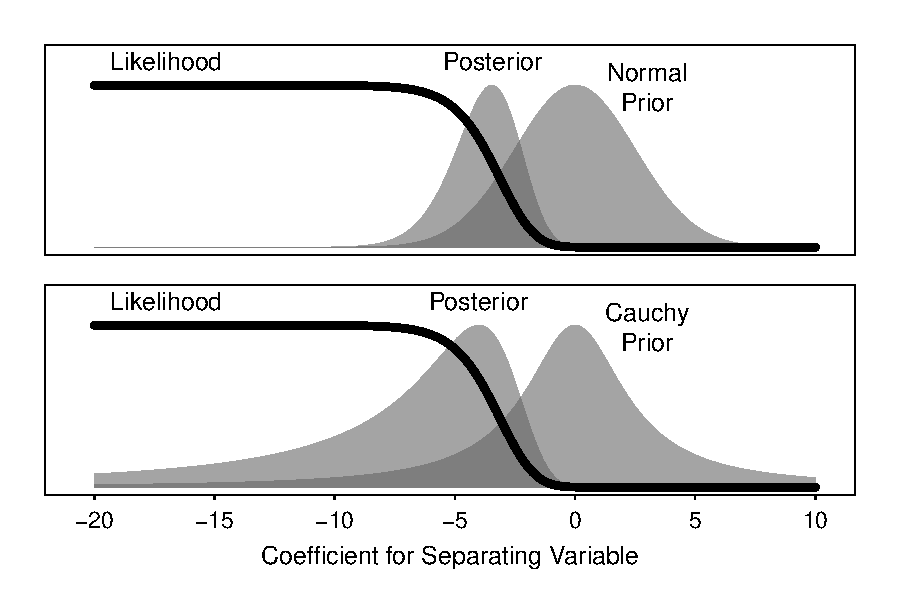
\includegraphics[scale = .8]{figs/thm-1-illustrated.pdf}
\caption{This figure provides an example monotonic likelihood, prior, and posterior that illustrate the key idea of Theorem \ref{thm:impact}. Notice that the likelihood is highly informative about the right-hand side of the posterior distribution, but not informative about the left-hand side of the posterior distribution. The choice of normal or Cauchy prior essentially determines the shape of the posterior in the direction of the separation.}\label{fig:thm-1-illustrated}
\end{center}
\end{figure}

Theorem \ref{thm:impact} simply implies that for large values of $\beta_s$ the posterior distribution depends almost entirely on the researcher's \emph{choice} of prior distribution. 
Thus, the choice of prior matters. 
While the choice of prior might not affect the conclusion about the \emph{direction} of the effect (i.e., one-sided credible interval), it has a large impact on the conclusion about the \emph{magnitude} of the effect (i.e., two-sided credible interval).
Credible intervals are crucial when discussing effect magnitudes (see \citealt{KingTomzWittenberg2000}; \citealt{Rainey2014a}; and \citealt{Gross2014}), and the choice of prior essentially drives the width of the credible interval.

\subsection*{The Impact of the Prior in Practice}

To illustrate the impact of the prior on inferences when dealing with separation, I replicate results from \cite{BarrilleauxRainey2014, barrilleaux-rainey-data}, who are interested in the effect of partisanship on governors' decisions to oppose the Medicaid expansion in their states under the Patient Protection and Affordable Care Act (ACA).
As the authors note, no Democratic governors opposed the expansion, which leads to separation. 
To see whether the choice of prior matters, I use MCMC to simulate from the posterior using Zorn's (\citeyear{Zorn2005}) and Gelman et al.'s (\citeyear{Gelmanetal2008}) suggested \emph{default} prior distributions. 

Figure \ref{fig:br-coef-illustrate-importance} shows the posterior medians and 90\% credible interval for the two default priors.\footnote{
The credible intervals I use throughout this paper are 90\% HPD credible intervals. 
One could define many intervals that have 90\% chance of containing the true parameter.
 However, the HPD interval is theoretically appealing because it is the \emph{shortest} of these intervals. 
 See \citet[esp. pp. 48-51]{Gill2008} and \citet[esp. p. 448]{CasellaBerger2002}. 
 An equal-tailed interval, one alternative to the HPD interval, tends to exacerbate the differences between the priors.} 
 While the choice of prior does not affect the conclusion about the \emph{direction} of the effect, it has a large impact on the conclusion about the \emph{magnitude} of the effect. 
 This can be especially important when researchers are making claims about the substantive importance of their estimated effects (see \citealt{KingTomzWittenberg2000}; \citealt{Rainey2014a}; and \citealt{Gross2014}). 
 For example, the Cauchy(0, 2.5) prior leads to a posterior median that is over 30\% larger in magnitude than the posterior median from Jeffreys' prior (-4.7 compared to -3.5). 
 The posterior mean is more than 70\% larger in magnitude using the Cauchy(0, 2.5) prior (-6.8 compared to -4.0). 
 Further, the 90\% credible interval is more than twice as wide for the Cauchy(0, 2.5) prior. 
 The choice between two \emph{default} priors leads to a large change in inferences.

\begin{figure}[H]
\begin{center}
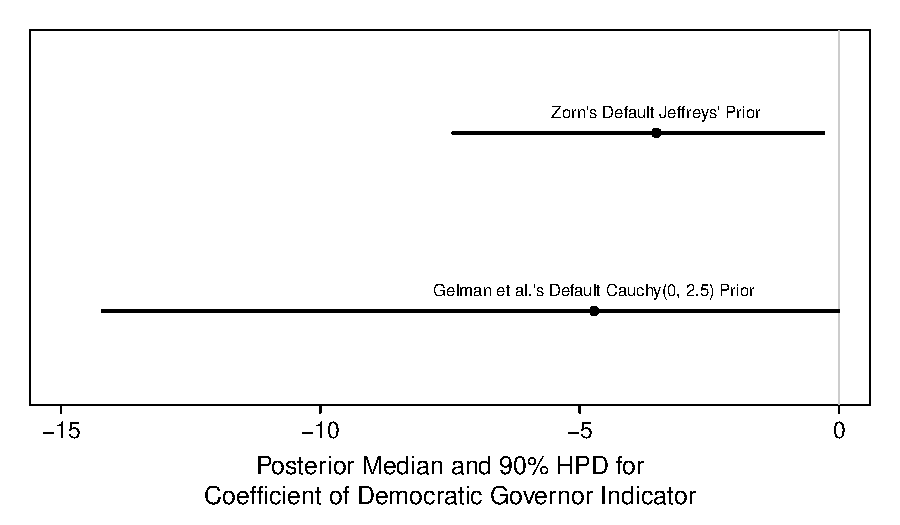
\includegraphics[scale = .8]{figs/br-coef-illustrate-importance.pdf}
\caption{This figure provides the posterior medians and 90\% credible intervals for the coefficient of the indicator for Democratic governors in the model used by \cite{BarrilleauxRainey2014}. 
Notice that Jeffreys' prior injects more information, as indicated by the smaller posterior median and credible interval. 
The credible interval using Cauchy(0, 2.5) prior is about \emph{twice} as wide as the credible interval using Jeffreys' prior. 
Further, the posterior median using the Cauchy(0, 2.5) prior is about 40\% larger in magnitude than the posterior median using Jeffreys' prior.}\label{fig:br-coef-illustrate-importance}
\end{center}
\end{figure}

Figure \ref{fig:bf-posterior-density-illustrate-importance} shows the posterior distribution for the coefficient of the indicator of Democratic governors. 
Notice that these two \emph{default} priors lead to different posterior distributions. 
In particular, the choice of the prior has a large impact on the right-hand side of the posterior, as suggested by Theorem \ref{thm:impact}. 
The more informative Jeffreys' prior leads to a more peaked posterior distribution that nearly rules out coefficients larger in magnitude than about -7. 
The less informative Cauchy(0, 2.5) prior leads to the conclusion that coefficients with much larger magnitudes, such as -15, are plausible. 
These differences are not trivial--there are large differences in the posterior distributions, and these differences can affect the conclusions that the researchers draw about the likely magnitude of the effect.

\begin{figure}[H]
\begin{center}
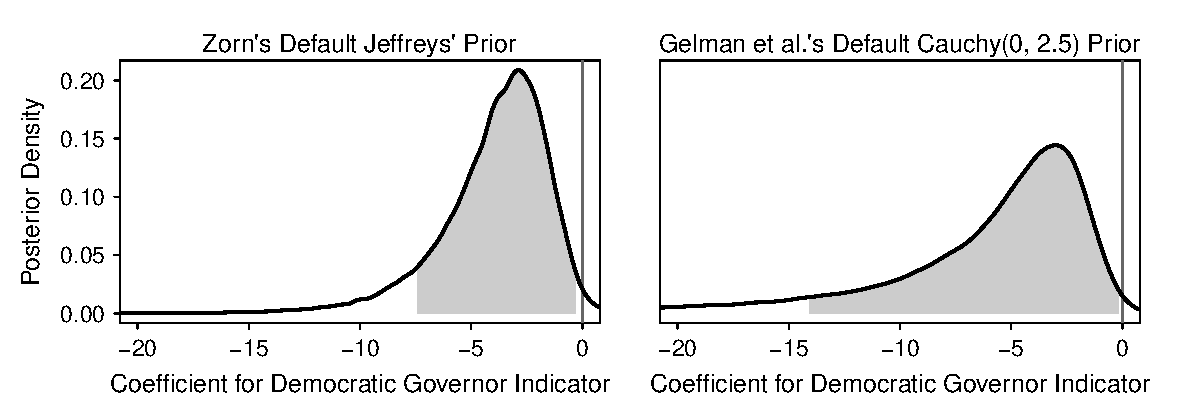
\includegraphics[scale = .8]{figs/br-posterior-density-illustrate-importance.pdf}
\caption{This figure shows the posterior distribution for the coefficient of the indicator for Democratic governors in the model offered by \cite{BarrilleauxRainey2014} for different default prior distributions. 
The grey shading indicates the 90\% credible interval. Notice that the location and the spread of the posterior depend on the prior chosen, especially the left-hand side of the distribution, as suggested by Theorem \ref{thm:impact}.}\label{fig:bf-posterior-density-illustrate-importance}
\end{center}
\end{figure}

\section*{Choosing an Informative Prior}

While is often sufficient to rely on default priors, this is not the case if one is interested in obtaining reasonable estimates and measures of uncertainty under separation. 
Indeed, in the replication of \cite{BarrilleauxRainey2014} above, I show that the overall posterior distribution, the width of the 90\% credible interval, and the posterior median largely depend on the prior one chooses. 
This implies that researchers relying on default priors alone risk under- or over-representing their confidence in the magnitude of the effect.

Data with separation fall into the category of ``weak data'' discussed by \cite{WesternJackman1994}--data that ``provide little information about parameters of statistical models.''
Under separation, the data simply offer no information about the upper-bound of the magnitude of the coefficient of the separating variable. 
Any reasonable regularization, then, must come in the form of an informative prior. 
%\citet[p. 38]{Leamer1983} writes: ``As I see it, the fundamental problem facing econometrics is how adequately to control the whimsical character of inference, how sensibly to base inferences on opinions when facts are unavailable.'' 
But a researcher's prior is not simply a spur-of-the-moment feeling. 
Instead, we should think of the prior as representing other information relevant to the estimation. 
This information can come from several sources, including quantitative studies of similar topics, detailed analyses of particular cases, and theoretical arguments.
As \citet[p. 415]{WesternJackman1994} note:
\begin{quote}
While extra quantitative information is typically unavailable, large and substantively rich stores of qualitative information from comparative and historical studies are often present but not available in a form suitable for analysis. 
Bayesian procedures enable weak quantitative information of comparative research to be pooled with the qualitative information to obtain sharper estimates of the regression coefficients.
\end{quote}
The best sources of prior information, though, depend on the substantive prior. 
The judgement of substantive researcher, based on their understanding of the substantive problem, is crucial.

When facing separation, I suggest researchers use a prior distribution that satisfies three properties:
\begin{enumerate}
\item \emph{Shrinks the estimates toward zero.} 
While the ultimate goal is to choose a prior distribution based on actual prior information, the prior distribution should also be appropriately conservative.
As mentioned before, the prior distribution largely drives the inferences in the direction of the separation. 
In this case, a non-central prior distribution in the direction of the separation has an especially large impact on the inferences. 
For this reason, I focus on prior distributions centered at zero to conservatively shrink coefficients toward zero \citep{GelmanJakulin2007}. 
The only choice the researcher needs to make is the amount of shrinkage appropriate for a given substantive problem.
\item \emph{Allows plausible effects.} 
The prior distribution should assign substantial prior probability to estimates that are \textit{a priori} plausible according to the researcher's prior information.
\item \emph{Rules out implausibly large effects.} 
The prior distribution should assign little prior probability to estimates that are \textit{a priori} implausible according to the researcher's prior information.\end{enumerate}

Different researchers will inevitably have different prior beliefs. 
For example, there is substantial disagreement among international relations theorists about the likely effects of nuclear weapons on conflict. 
Some optimists believe that nuclear weapons make peace much more likely. 
\citet[p. 57]{Mearsheimer1993} argues that ``nuclear weapons are a powerful force for peace'' and observes:
\begin{quote}
In the pre-nuclear world of industrialized great powers, there were two world wars between 1900 and 1945 in which some 50 million Europeans died. In the nuclear age, the story is very different. Only some 15,000 Europeans were killed in minor wars between 1945 and 1990, and there was a stable peace between the superpowers that became increasingly robust over time. A principal cause of this ``long peace'' was nuclear weapons.
\end{quote}
\citet[p. 283]{BDMRiker1982} even theorize that the probability of conflict ``decreases to zero when all nations are nuclearly armed.'' 

On the other hand, some pessimists (e.g., \citealt{Sagan1994}) believe that nuclear weapons do not deter conflict, only make it more catastrophic. 
\citet[pp. 68-69]{Mueller1988} writes: 
\begin{quote}
Nuclear weapons may well have enhanced this stability--they are certainly dramatic reminders of how horrible a big war could be. But it seems highly unlikely that, in their absence, the leaders of the major powers would be so unimaginative as to need such reminding. Wars are not begun out of casual caprice or idle fancy, but because one country or another decides that it can profit from (not simply win) the war--the combination of risk, gain, and cost appears to be preferable to peace. Even allowing considerably for stupidity, ineptness, miscalculation, and self-deception in these considerations, it does not appear that a large war, nuclear or otherwise, has been remotely in the interest of essentially-contented, risk-averse, escalation-anticipating powers that have dominated world affairs since 1945.
\end{quote}

The optimists and the pessimists have different prior beliefs about the likely effects nuclear weapons. 
These different beliefs must lead to different interpretations of the evidence because the prior distribution has such a strong impact on the posterior distribution in the direction of the separation. 
Because of this, researchers must clearly communicate the dependence of the inferences on the choice of prior by transparently developing an informative prior distribution and providing the inferences for alternative prior beliefs.

However, choosing a prior distribution is quite difficult, especially for multidimensional problems. 
\cite{GillWalker2005} provide an overview of methods of choosing a prior appropriate to social science research. 
However, the most sensible approach for choosing a prior distribution depends on the nature of the statistical model and the prior information.

In general, the researcher might assess the reasonableness of the prior distribution by examining the prior distribution and asking herself whether the prior and model produce a distribution for the quantities of interest that matches her prior information. 
Under the Bayesian framework, the researcher has a fully specified model $\pi_{new} = p(y_{new}|\beta)p(\beta)$ and can simulate the quantity of interest $q_{new} = q(\pi_{new})$ from the model \textit{prior to observing the data}. 
This works much like the Clarify algorithm \citep{KingTomzWittenberg2000}.
By repeatedly simulating from the prior distribution $\tilde{\beta} \sim p(\beta)$, calculating $\tilde{\pi}_{new} = p(y_{new}|\tilde{\beta})$, and calculating $\tilde{q}_{new} = q(\tilde{\pi}_{new})$, the researcher can recover the transformed prior distribution of $q_{new}$.
Just as a researcher can use simulation to interpret the coefficient estimates of nonlinear models, she can use simulation to interpret the prior distribution.

This simulation is entirely pre-data. 
The researcher does not need to fit the model to data to simulation the quantities of interest. 
Instead, she can simulate from the prior distribution (rather than the posterior), and use these prior simulations to interpret the prior distribution.

However, it is difficult to work with more than one dimension of the prior distribution. 
Specifying the full prior distribution requires simultaneously choosing prior distributions for the coefficients of the $k + 1$ explanatory variables, as well as the relationships among these coefficients (e.g., family, location, scale, and correlations of each coefficient). 
This process is intractably tedious, because the researcher must evaluate the prior for each combination of each parameter set at a range of values. 
Even if the researcher considers only independent normal priors centered at zero and only ten values for each scale, then the researcher must examine $10^{k+1}$ prior distributions. 
If the researcher has eight control variables, so that $k = 8$, (e.g., \citealt{BarrilleauxRainey2014}), then the researcher must evaluate one \emph{billion} prior distributions.

But only specific regions of the $k + 1$ dimensional prior distribution are practically important when addressing separation. 
This allows the researcher to dramatically simplify the choice of prior. 
In particular, the researcher can simplify the focus in two specific ways.
\begin{enumerate}
\item \emph{Focus only on the separated coefficient.} 
Since the data swamp the prior for all the model coefficients except $\beta_s$, the only relevant ``slices'' of the prior distribution are those in which all other coefficients are near their maximum likelihood estimates.
\item \emph{Focus in the direction of the separation.} 
The likelihood also swamps the prior in the direction opposite the separation. 
Unless the researcher has an extremely small data set (i.e., smaller than \cite{BarrilleauxRainey2014}, who have $N = 50$), then the likelihood essentially rules out values less [greater] than zero when the direction of separation is positive [negative].
\end{enumerate}
\noindent I refer to this simplified focus as the \emph{partial} prior distribution. 

Formally, we might write the partial prior distribution as $p^*(\beta_s | \beta_s \geq 0, \beta_{-s} = \hat{\beta}_{-s}^{mle})$ when $\hat{\beta}^{mle}_s = +\infty$ and $p^*(\beta_s | \beta_s \leq 0, \beta_{-s} = \hat{\beta}_{-s}^{mle})$ when $\hat{\beta}^{mle}_s = -\infty$.
Much like the researcher can recover the prior distribution of $q_{new}$ implied by the prior distribution, she can recover the distribution of $q_{new}$ implied by the \textit{partial} prior distribution by repeatedly simulating from the \textit{partial} prior distribution $\tilde{\beta}^* \sim p^*(\beta_s | \beta_s \leq 0, \beta_{-s} = \hat{\beta}_{-s}^{mle})$, calculating $\tilde{\pi}^*_{new} = p(y_{new}|\tilde{\beta}^*)$, and calculating $\tilde{q}^*_{new} = q(\tilde{\pi}^*_{new})$.

The researcher should only the partial prior distribution to study and interpret the prior distribution, not to estimate the model. 
For estimating the model, researchers should use the full prior distribution described below in the section ``Estimating the Full Model.''

This process requires the researcher to use the data twice---an initial fit using maximum likelihood and a final fit using MCMC. 
First, the researcher fits the model using maximum likelihood to obtain a reasonable estimate of the coefficients or the non-separating explanatory variables (upon which the quantities of interest depend). 
The maximum likelihood estimation produces an estimate of $\approx \pm \infty$ for the coefficient of the separation variable; this is akin to excluding the perfectly predicted cases from the analysis or using the imperfectly predicted cases to estimate the coefficients of the non-separated explanatory variables.  
For example, even though no Democratic governors opposed the Medicaid expansion, \cite{BarrilleauxRainey2014} can use the Republican states to estimate the coefficients for their other explanatory variables, including the percent of the state's residents who feel favorable toward the ACA, whether Republicans control the state legislature, the percent of the state that is uninsured, and others.
This initial maximum likelihood estimation only serves to identify the especially important region of the (multivariate) prior distribution: the dimension for the coefficient of the separating explanatory variable in the direction of the separation with the other coefficients near their maximum likelihood estimates.

For example, \cite{BarrilleauxRainey2014} do not need to use prior information to obtain reasonable estimates for their measures of need and public opinion. 
Further, because no Democratic governors opposed the Medicaid expansion, they do not need the prior to rule out large \textit{positive} effects for Democratic partisanship. 
In these cases, the likelihood is sufficiently informative. However, \cite{BarrilleauxRainey2014} do need to use the prior to rule out large \textit{negative} effects for Democratic partisanship, because the likelihood cannot effectively rule out implausibly large negative effects. 
Indeed, the likelihood is monotonically decreasing in the coefficient of the indicator of Democratic governors. 
That is, the likelihood increases as the coefficient of Democratic partisanship becomes more negative. 
The larger the negative effect, the more likely separation would occur. 
The usual maximum likelihood estimator, therefore, provides implausibly large negative estimates and unreasonable standard errors. 
Theorem \ref{thm:impact} provides a more formal treatment of this intuition, but prior information is essential to obtain reasonable estimates and measures of uncertainty. 

Choosing a prior, though, requires thoughtful effort. 
As I show above, default priors can lead to much different conclusions, so it is essential to build actual prior information into the model. 
In order to choose a reasonable, informative prior distribution, researchers can use simulation to obtain the partial prior distribution of the quantity of interest.
The following steps describe how researchers can simulate from the partial prior distribution of a quantity of interest and use the simulations to check the reasonableness of the choice.
\begin{enumerate}
\item Estimate the model coefficients using maximum likelihood, giving the coefficient vector $\hat{\beta}^{mle}$. 
Include the separating variable $s_i$ in the model. 
Of course, this leads to implausible estimates for $\beta_s$, but the purpose is to choose reasonable values at which to fix the \emph{other} coefficients in order to focus on a single slice of the full prior. 
\item Choose a prior distribution $p(\beta_s | \sigma)$ for the separating variable $s$ that is centered at zero with scale parameter $\sigma$. 
One sensible choice is the scaled $t$ distribution, which has the normal and Cauchy families as special cases ($\text{df} = \infty$ and $\text{df} = 1$, respectively). 
\item Choose a large number of simulations $n_{sims}$ to perform (e.g., $n_{sims} \geq 10,000$) and for $i$ in 1 to $n_{sims}$, do the following:
	\begin{enumerate}
	\item Simulate $\tilde{\beta}^{[i]}_s \sim p(\beta_s)$.
	\item Replace $\hat{\beta}_s^{mle}$ in $\hat{\beta}^{mle}$ with $\tilde{\beta}^{[i]}_s$, yielding the vector $\tilde{\beta}^{[i]}$.
	\item Calculate and store the quantity of interest $\tilde{q}^{[i]} = q\left(\tilde{\beta}^{[i]}\right)$. 
	This quantity of interest might be a first-difference or risk-ratio, for example.
	\end{enumerate}
\item Keep only those simulations in the direction of the separation (e.g., $\tilde{\beta}_s^{[i]} \geq 0$ when $\hat{\beta}_{s}^{mle} = +\infty$ and $\tilde{\beta}_s^{[i]} \leq 0$ when $\hat{\beta}_{s}^{mle} = -\infty$).\footnote{In some situations, researchers may wish to skip this step. For example, if the number of perfectly predicted cases (e.g., states with Democratic governors or nuclear dyads) are relatively few, then the researchers can skip this step to evaluate the prior in the direction of the separation as well as the opposite direction. However, a scale parameter that produces reasonable prior distribution in the direction of the separation should usually also lead to a reasonable prior distribution in the direction opposite the separation. In most cases, though, the likelihood is informative that the coefficient is probably in the same direction of the separation, so excluding simulations in the opposite direction of the separation simplifies the process.}
\item Summarize the simulations $\tilde{q}$ using quantiles, histograms, or density plots. 
If the prior is inadequate, then update the prior distribution $p(\beta_s | \sigma)$ by choosing a larger or smaller value of $\sigma$.
\end{enumerate}

Given that the inference can be highly dependent on the choice of prior, I recommend that the researcher choose at least three prior distributions: (1) an \emph{informative} prior distribution that represents her actual information, (2) a highly \emph{skeptical} prior distribution that suggests the effect is likely small, and (3) a highly \emph{enthusiastic} prior that suggests the effect might be very large. 
Indeed, \citet[p. 422]{WesternJackman1994} note: 
\begin{quote}
Still, the subjective choice of prior is an important weakness of Bayesian practice. The consequences of this weakness can be limited by surveying the sensitivity of conclusions to a broad range of prior beliefs and to subsets of the sample.
\end{quote}
Combined with Zorn's (\citeyear{Zorn2005}) and Gelman et al.'s (\citeyear{Gelmanetal2008}) suggested defaults, these provide a range of prior distributions that the researcher can use to evaluate her inferences.

\section*{Estimating the Full Model}

Once the researcher obtains a reasonable prior distribution as well as several to use for robustness checks, she can use MCMC \citep{Jackman2000} to obtain simulations from the posterior. 
\cite{Zorn2005} and \cite{Gelmanetal2008} suggest variations on maximum likelihood to quickly obtain estimates and confidence intervals, but the normal approximation typically used to simulate the parameters and calculate quantities of interest \citep{KingTomzWittenberg2000} is particularly inaccurate under separation \citep{HeinzeSchemper2002}. 
As an alternative, I recommend the researcher use MCMC to simulate directly from the posterior distribution. 
The researcher can then use these simulations to calculate point estimates and confidence intervals for any desired quantity of interest. 
For the informative $p_{\text{inf}}(\beta_s)$, skeptical $p_{\text{skep}}(\beta_s)$, and enthusiastic $p_{\text{enth}}(\beta_s)$ priors , I suggest the model:

\begin{equation}
Pr(y_i =1) = \text{logit}^{-1}(\beta_{cons} + \beta_s s_i +  \beta_1 x_{i1} + \beta_2 x_{i2} + ... + \beta_k x_{ik})
\end{equation}
\begin{equation}
\beta_s \sim  p_m(\beta_s) \text{, for } m \in \{\text{inf, skep, enth}\},
\end{equation}
with improper, constant priors on the other model coefficients. 
Because the researcher is not choosing the prior based on the desirable or undesirable features of the \textit{posterior}, inference can proceed in the usual way after the MCMC estimation.


\section*{Application: Nuclear Proliferation and War}

A recent debate emerged in the conflict literature between \cite{Rauchhaus2009} and \cite{BellMiller2015} that revolves around the issue of separation. 
\citet[p. 262]{Rauchhaus2009} hypothesizes that ``[t]he probability of major war between two states will decrease if both states possess nuclear weapons.'' 
Summarizing his empirical results, Rauchhaus writes:
\begin{quote} 
The hypotheses on nuclear symmetry find strong empirical support. The probability of a major war between two states is found to decrease when both states possess nuclear weapons (p. 269).
\end{quote}

Despite using the same data, \citet[p. 9]{BellMiller2015} claim that ``symmetric nuclear dyads are not significantly less likely to go to war than are nonnuclear dyads.'' 
Their disagreement hinges, in part, on whether and how to handle separation, because no nuclear dyad in Rauchhaus data engages in war.\footnote{
\cite{BellMiller2015} also disagree with Rauchhaus' (\citeyear{Rauchhaus2009}) coding of the 1999 conflict in Kargil between India and Pakistan, which both possessed nuclear weapons. 
This conflict is excluded from Rauchhaus' data set, but Bell and Miller argue that it should be included as a war between two nuclear-armed states, eliminating the problem of separation.} 
\cite{Rauchhaus2009} ignores the separation and estimates that nonnuclear dyads are about 2.7 million times more likely to go to war than symmetric nuclear dyads.
\cite{BellMiller2015}, on the other hand, use Jeffreys' (\citeyear{Jeffreys1946}) invariant prior, as suggested by \cite{Zorn2005}, and estimate that nonnuclear dyads are only about 1.6 times more likely to engage in war. 
Because these authors use very different prior distributions, they reach very different conclusions.\footnote{
\cite{Rauchhaus2009} does not use a formal prior distribution, but uses generalized estimating equations, which we might interpret as having an improper, uniform prior on the logistic regression coefficients from minus infinity to plus infinity. 
The estimate is finite only due to a stopping rule in the iterative optimization algorithm.} 
This raises important questions. 
\begin{enumerate}
\item First, would a reasonable, informative prior distribution support Rauchhaus' position of a meaningful effect or Bell and Miller's position of essentially no effect? 
\item Second, how robust is the conclusion to a range of more and less informative prior distributions?
\end{enumerate}
To address these questions, I re-analyze these data \citep{bell-miller-data} with special attention the to the prior distribution.

\subsection*{Prior}

The first step in dealing with the separation in a principled manner is to choose a prior distribution that represents actual prior information. 
To choose a reasonable prior, I follow the process above to generate a partial prior distribution for the risk-ratio that \cite{BellMiller2015} emphasize. 
I experimented with a range of prior distributions, from a variety of families, but settled on a normal distribution with mean zero and standard deviation 4.5. 
This serves as an informative prior and represents my own prior beliefs.   
I chose this prior distribution because it essentially rules out risk-ratios larger than 1,000--effects that I find implausibly large--and treats risk-ratios smaller than 1,000 as plausible. 
Figure \ref{fig:bm-ppd-hist} and Table \ref{tab:bm-ppd-deciles} summarize the partial prior distributions for the this normal distribution with standard deviation 4.5.

To evaluate the robustness of any statistical claims to the choice of prior, I also selected a highly skeptical and highly enthusiastic prior. 
I chose a normal distribution with mean zero and standard deviation two to serve as a skeptical prior that represents the belief that any pacifying effect of nuclear weapons is small (e.g., \citealt{Mueller1988}). 
This skeptical prior distribution essentially rules out risk-ratios larger than 25 as implausibly large. 
Finally, I selected a normal distribution with mean zero and standard deviation eight to serve as an enthusiastic prior that represents the belief that the pacifying effects of nuclear weapons might be quite large (e.g., \citealt{Mearsheimer1993}). 
This enthusiastic prior, on the other hand, treats risk-ratios as large as 500,000 as plausible. 
Figure \ref{fig:bm-ppd-hist} shows the partial prior distributions for the informative, skeptical, and enthusiastic prior distributions. 
For convenience, Table \ref{tab:bm-ppd-deciles} provides the deciles of the partial prior distributions shown in Figure \ref{fig:bm-ppd-hist}. 

\begin{figure}[H]
\begin{center}
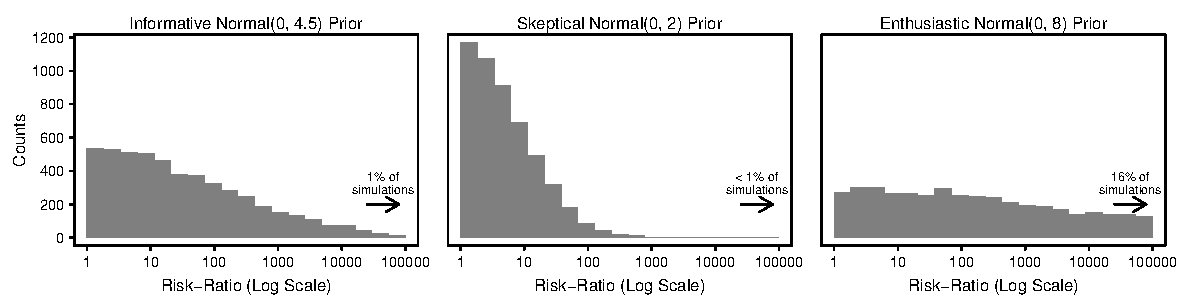
\includegraphics[scale = .8]{figs/bm-ppd-hist.pdf}
\caption{This figure shows the partial prior distribution for the risk-ratio of war in nonnuclear dyads to nuclear dyads. 
The risk-ratio tells us how many times more likely war is in nonnuclear dyads compared to nuclear dyads. 
Notice that the informative prior treats effects smaller than about 1,000 as plausible, but essentially rules out larger effects. 
The skeptical prior essentially rules out effects larger than 25, while the enthusiastic prior treats effects between 1 and 100,000 as essentially equally likely.}\label{fig:bm-ppd-hist}
\end{center}
\end{figure}

% latex table generated in R 3.1.1 by xtable 1.7-3 package
% Sun Oct  5 07:07:18 2014
\begin{table}[H]
\centering
{\scriptsize
\begin{tabular}{|cccccccccc|}
  \hline
 & 10\% & 20\% & 30\% & 40\% & 50\% & 60\% & 70\% & 80\% & 90\% \\ 
  \hline
Informative Normal(0, 4.5) Prior &       1.7 &       3.1 &       5.6 &      10.3 &      19.5 &      44.1 &      98.8 &     296.9 &   1,577.7 \\ 
  Skeptical Normal(0, 2) Prior &       1.3 &       1.7 &       2.2 &       2.9 &       3.9 &       5.4 &       8.3 &      13.2 &      26.7 \\ 
  Enthusiastic Normal(0, 8) Prior &       2.9 &       8.1 &      24.7 &      76.5 &       256 &     987.6 &   5,300.9 &  42,466.7 & 643,954.6 \\ 
   \hline
\end{tabular}
}
\caption{This table provides the deciles of the prior predictive distribution for the 
                  risk-ratio of war in nonnuclear and nuclear dyads. The risk-ratio
                  tells us how many times more likely war is in non-nuclear dyads compared 
                  to nuclear dyads. Notice that the informative prior suggests a median 
                  risk-ratio of about 20, which is a large, but plausible, effect. The skeptical prior suggests a median 
                  ratio of about 4 and the enthusiastic prior suggests a median ratio of over 
                  200.} 
\label{tab:bm-ppd-deciles}
\end{table}


Notice that the skeptical prior suggests that risk-ratios above and below 4 are equally likely (i.e., 50th percentile of the partial prior distribution is 3.9), while the enthusiastic prior suggests that effects above and below 220 are equally likely. 
The informative prior, on the other hand, suggests (more reasonably, in my view) that the effect is equally likely to fall above and below 20. 
These three prior distributions, along with the defaults suggested by \cite{Zorn2005} and \cite{Gelmanetal2008}, provide a range of distributions to represent a range of prior beliefs.

\subsection*{Posterior}

Figure \ref{fig:bm-posterior-density} shows the posterior distributions for the coefficient of the indicator of nuclear dyads using the informative, skeptical, enthusiastic, and two default prior distributions. 
The areas shaded grey indicate the 90\% credible intervals. Notice that the location (e.g., peak or mode), shape, scale, and credible interval depend on the choice of prior. 
While the magnitude of this coefficient is not easily interpretable, notice that Gelman et al.'s (\citeyear{Gelmanetal2008}) suggested default prior is somewhat similar to the informative prior, but Zorn's (\citeyear{Zorn2005}) suggested default is quite similar to the \emph{skeptical} prior. 
Thus, these distributions illustrate that the prior is important when dealing with separation. 
Indeed, it is a critical step in obtaining reasonable inferences.

\begin{figure}[H]
\begin{center}
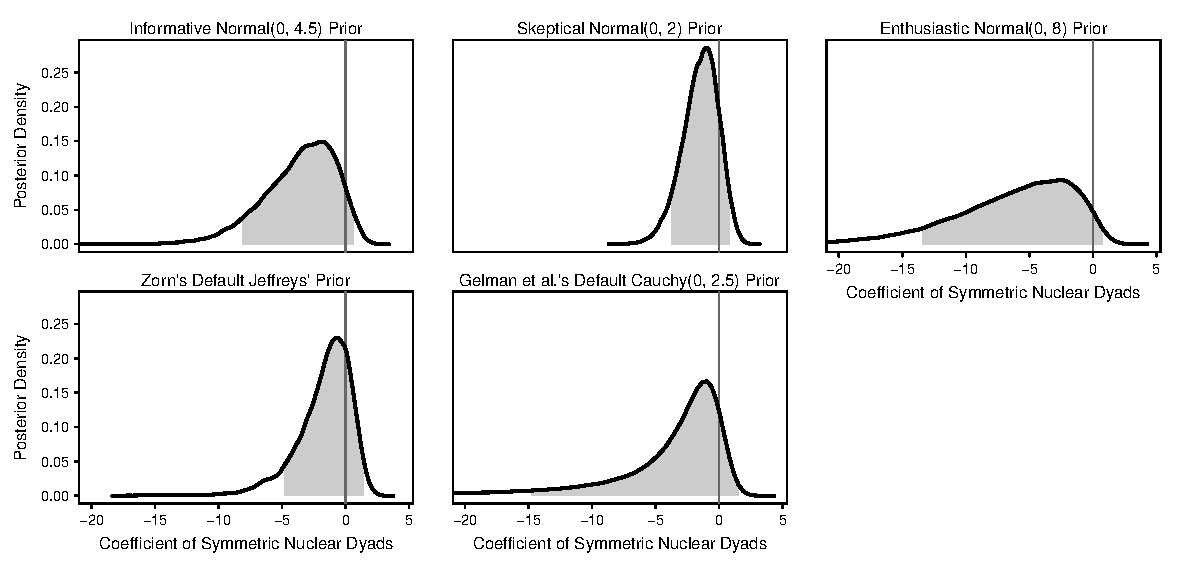
\includegraphics[scale = .8]{figs/bm-posterior-density.pdf}
\caption{This figure shows the posterior distribution for the logit coefficient of the indicator of nuclear dyads using each of the five prior distributions.  
The grey shading indicates the 90\% credible interval. 
Notice that the choice of prior has a large effect on the inferences. 
For example, the using the enthusiastic prior suggests the coefficient might be as large as -13, while using the skeptical prior suggests the coefficient is probably not larger than -4. 
Importantly, notice the similarity between the posterior using Zorn's (\citeyear{Zorn2005}) suggested default prior and the skeptical prior, in terms of their peak (i.e., mode), shape, and credible interval.}\label{fig:bm-posterior-density}
\end{center}
\end{figure}

I now turn to the posterior distribution of the risk-ratios--the key quantity of interest in the debate between \cite{BellMiller2015} and \cite{Rauchhaus2009}. 
Figure \ref{fig:bm-rr} presents the posterior medians and the 90\% credible intervals for each prior. 
An initial glance at the figure shows substantial variation in the point estimates and the width of the intervals. 
However, these risk-ratios and credible intervals are plotted on the log scale (otherwise the wider intervals dominate the plot), so the figure tends to \textit{understate} the variation in the inferences across priors. 
Notice that the informative prior suggests the true risk-ratio has about a 90\% chance of falling between about 0.1 and about 2000, with a posterior median of about 25.
The skeptical prior, on the other hand, suggests the risk-ratio has about a 90\% chance of falling between 0.1 and 30, with a posterior median of about 4. 
The enthusiastic prior suggests the risk-ratio has about a 90\% chance of falling between 0.1 and 500,000. 
The inferences from these priors are \emph{very} different. 

Further, the 90\% credible interval using Zorn's (\citeyear{Zorn2005}) default is \emph{much} narrower than the informative prior, and the posterior median of Zorn's suggested default prior is even smaller than the \emph{skeptical} prior. 
For this particular application, Gelman's suggested default more closely matches the informative prior, though notice that the point estimate from Gelman's prior is 62\% smaller than that from the informative prior and the upper-bound of the credible interval is 13 times larger.

\begin{figure}[H]
\begin{center}
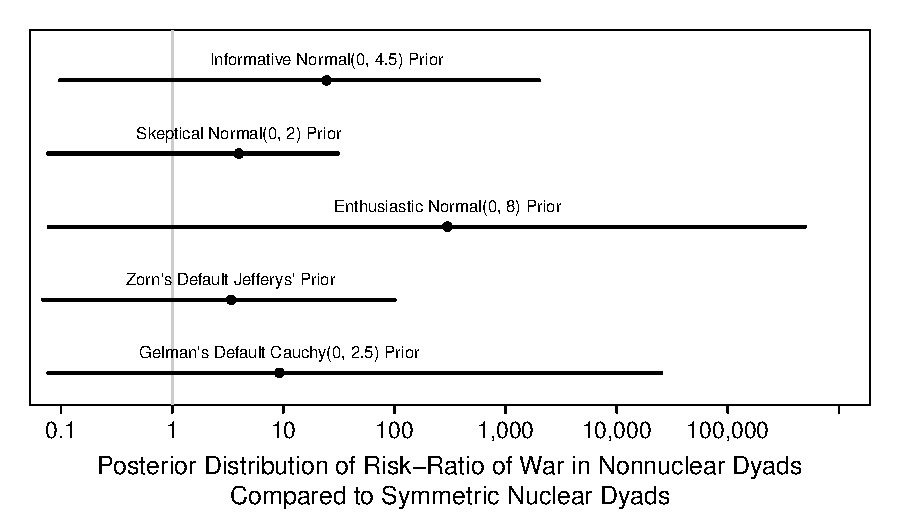
\includegraphics[scale = .8]{figs/bm-rr.pdf}
\caption{This figure shows the posterior median and 90\% credible intervals for the risk-ratio using each of the five prior distributions \emph{on the log scale}. 
Notice that the choice of prior has a huge effect on the inferences about the risk-ratio. 
For example, the skeptical prior suggests the ratio might be as large as 31, while the enthusiastic prior suggests the ratio might be as large as 500,000. 
Also, notice that the posterior median from Zorn's proposed default prior is \emph{smaller} than the posterior median from the skeptical prior.}\label{fig:bm-rr}
\end{center}
\end{figure}

Finally, I use the posterior distributions from each prior to calculate the probability that the presence of nuclear weapons make war less likely (i.e., the probability that the risk-ratios shown in Figure \ref{fig:bm-rr} are greater than one). 
Recall Rauchhaus' hypothesis that nuclear weapons decrease the chance of war. 
These probabilities can be thought of as the probability that Rauchhaus' hypothesis is correct. 
Following the standard of $p \leq 0.05$ as offering strong evidence against the null hypothesis, it is reasonable to take $Pr(RR > 1) \geq 0.95$ as strong evidence for the research hypothesis. 
Figure \ref{fig:bm-pr-hypothesis} shows the probability that the hypothesis is correct for each prior distribution. 
Notice that while only the enthusiastic prior falls above the 0.95 standard, the evidence for the claim is at least suggestive. 
Perhaps most importantly for my purposes, Zorn's suggested default leads to the \emph{least} evidence in favor of Rauchhaus' hypothesis--even the skeptical prior provides more evidence for Rauchhaus' claim.

\begin{figure}[H]
\begin{center}
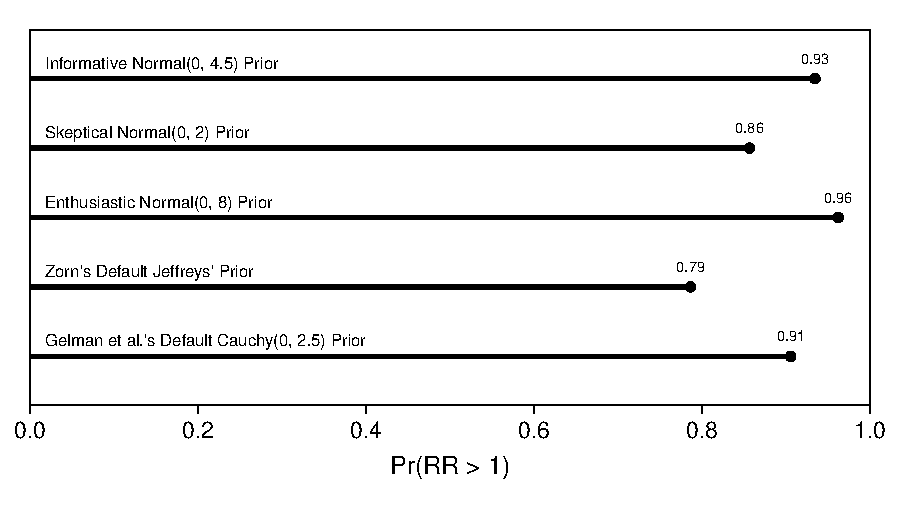
\includegraphics[scale = .8]{figs/bm-pr-hypothesis.pdf}
\caption{This figure shows the posterior probability of the hypothesis that nonnuclear dyads are \emph{more} likely to engage in war than symmetric nuclear dyads for each of the five prior distribution. 
From a hypothesis testing perspective, the evidence for the hypothesis is borderline or suggestive for each prior. 
However, notice that the skeptical prior, perhaps held by a researcher who believes the pacifying effect of nuclear weapons is small or nil, yields \emph{greater} evidence for the hypothesis than Jeffreys' invariant prior suggested as a default by \cite{Zorn2005}.}\label{fig:bm-pr-hypothesis}
\end{center}
\end{figure}

\subsection*{Conclusion}

Separation is a relatively common situation in political science. 
It is also an unusual ``problem'' because the effects in the sample are ``too big'' for maximum likelihood. 
In this situation, dropping the separating variables (i.e., deliberate specification bias) or interpreting the implausible coefficients and standard errors are particularly unattractive options. 
But even the most principled solution to date, the incorporation of prior information via default priors (\citealt{Zorn2005} and \citealt{Gelmanetal2008}), has shortcomings.

First, the normal approximations necessary to simulate quantities of interest after using these methods perform poorly. 
While it is possible to use profile likelihood methods to obtain more accurate confidence intervals for the coefficients (\citealt{Zorn2005}, \citealt{HeinzeSchemper2002}, and \citealt{McCullaghNelder1989}), it is difficult to translate these intervals into confidence intervals for quantities of interest. 
I provide the computational tools to simulate directly from the posterior using both Zorn's (\citeyear{Zorn2005}) and Gelman et al.'s (\citeyear{Gelmanetal2008}) suggested default priors.

Second, the applications examining the effect of nuclear weapons and the effect of governors' partisanship illustrate what Theorem \ref{thm:impact} proves--under separation, the choice of prior affects substantive conclusions. 
Even the predominant default priors used to deal with separation can provide very different inferences. 
A carefully-chosen, informative prior is an essential step in the process of obtaining reasonable inferences when dealing with separation. 
But what does this mean for applied researchers? 
I suggest two implications:
\begin{enumerate}
\item When facing separation, the choice of prior matters. 
Researchers must carefully choose a prior that represents actual prior information. 
Otherwise, the point and interval estimates will be too small or too large.
\item In addition to carefully choosing an informative prior that represents her own beliefs, the researcher should show how the inferences change for a range of prior distributions. 
In the debate between \cite{BellMiller2015} and \cite{Rauchhaus2009}, the choice of prior almost completely drives the inferences about the likely magnitude of the risk-ratio. 
Thus, to the extent that there is disagreement about the prior, there will be disagreement about the results. 
In particular, I suggest that in addition to focusing on an informative prior, researchers report the key quantities of interest for a skeptical prior, an enthusiastic prior, and the two default priors suggested by \cite{Zorn2005} and \cite{Gelmanetal2008}.
\end{enumerate}

When facing separation, researchers must \emph{carefully} choose a prior distribution to nearly rule out implausibly large effects. 
This paper introduces the concept of a partial prior distribution and the associated computational tools to help researchers choose a prior distribution that represents actual prior information for their particular research problem. 
By presenting results using several prior distributions, including an informative prior, researchers can increase the transparency, credibility, and accuracy of their inferences when dealing with separation.

%\clearpage
\singlespace
\bibliographystyle{apsr_fs}
\bibliography{bibliography.bib}

\end{document}



